Before going deep into structural properties of decomposable digraphs we first need to establish what a graph is.
For some graph $G(V,E)$ where $V$ and $E$ are two sets contaning the \textbf{vertices} (also commonly called nodes) and \textbf{egdes} of the graph respectivlely.
%Example $V=\lbrace a,b,c \rbrace$ then $a,\ b$ and $c$ are three distinct vertices of the graph $G$ and the only vertices of $G$.
We define the \textbf{size} of the graph to be the number of vertices $|V|$ this is also known as \textbf{cardinality} of $V$.
%In the case of the example the size of $G$ $|V|=3$ it is also called the order of a graph.
An \textbf{edge} $e \in E$ is where $e \equiv (a, b)$ and $\{ a, b \} \subseteq V$ we then say $e$ is an edge in $G$, $e$ is in this case called \textbf{incedent} to $a$ and $b$. 
We call $a,b \in V$ \textbf{adjecent} if there is an edge $(a,b)$ or $(b,a)$ (two given vertices connected by an edge is said to be adjecent).
If an edge goes from and to the same vertex $(a,a)$ it is called a \textbf{loop}.
The set of edges $e_1, \dots, e_k$ is usally describe whit the letter $E$ where each edge contains a pair of vertices that are adjecent. The letter $V$ is to denoted the set of vertices in the given graph. \\
In a graph we have something called a \textbf{walk} which is a repeting ordering of vertices an edges in the graph $G$ where the edge in between the two vertices in the ordering is an edge between the vertices in $G$ (for $(a,e_1,b)$ to be a walk the edge $e_1$ has to be between $a$ and $b$). by repeting it means that a vertex can apear twice in a walk.
We call a walk closed if the first vertex in the walk is the same as the last.\\
Every vertex $v\in V$ of $G(V,E)$ have a \textbf{degree} denoted $d(v)$ which is the number of incident edges to $v$.
A \textbf{path} in a graph is a walk where each vertex in the ordering can only apear one time. 
A \textbf{cycle} is a closed walk where the only vertex pressent more then one time is the first vertex( also called a closed path). 
Let $X$ be a subset of the vertices $X\subseteq V$ then we say that $V\backslash X$ is the set of vertices with out the vertices in $X$, i.e. $V\backslash X \equiv V-X$. 
A subgraph $H$ of $G$ can contain any of the vertices and the arcs connected to the chossen vertecies in H. 
you can not have an edge conecting no vertices in $H$ but you do not have to choose all the arcs in $G$ between the chossen vertices in $H$ for $H$ to be a subgraph. \\
As we can look at subsets we sometimes need to look at sub-paths, for a path $P=x_1\dots x_k$ a \textbf{sub-path} is a path $P'=x_i\dots x_j$ of $P$ where $1\leq i < j \leq k$.
%The describe example can be seen in figure \autoref{fig:graph}.
\begin{figure}[!h]
    \begin{subfigure}{0.48\textwidth}
        \centering
        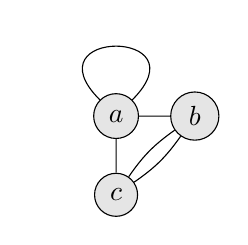
\begin{tikzpicture}
            [main/.style ={draw,circle}]
            \node[main][fill=gray!20!white] (a){$a$};
            \node[main][fill=gray!20!white] (b)[right of = a]{$b$};
            \node[main][fill=gray!20!white](c)[below of= a]{$c$};
            \draw (a) to (b) (c) to (a) (c) to [bend right =10](b) (c) to [bend left =10](b); 
            \draw (a) to [loop,red] (a);
        \end{tikzpicture} 
        \caption{graph $G(V,E)$ is an example of a graphs, the red edge is a loop, and all pair of vertices in this graph is adjecent.}
        \label{fig:graph}
    \end{subfigure}\hfill
   \begin{subfigure}{0.48\textwidth}
    \centering
        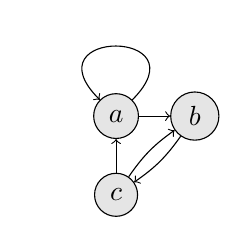
\begin{tikzpicture}
            [main/.style ={draw,circle}]
            \node[main][fill=gray!20!white] (a){$a$};
            \node[main][fill=gray!20!white] (b)[right of = a]{$b$};
            \node[main][fill=gray!20!white](c)[below of= a]{$c$};
            \draw[->] (a) to (b);
            \draw[->](c) to (a);
            \draw[->](c) to [bend left =10](b);
            \draw[->](b) to [bend left =10](c); 
            \draw[->] (a) to [loop,red] (a);
        \end{tikzpicture} 
        \caption{This is an oriantation of the edges in the graph which makes this a digraph}
        \label{fig:digraph}
   \end{subfigure}
\end{figure}


Before delving more specific into graphs and digraphs we must establish some important prerequisite and properties. 
A graph is called \textbf{simple} if there is no loops and no multiple edges. 
With multiple edges it means multiple edges between the same pair of vertices like in \autoref{fig:graph} between $b$ and $c$.
\begin{figure}[!h]
	\centering
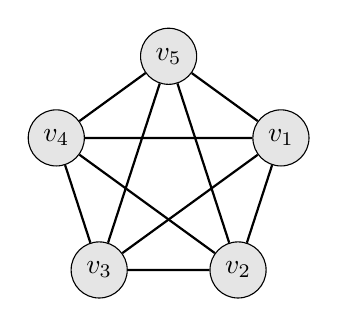
\begin{tikzpicture}[
	xs/.style = {xshift=#1 mm},
	ys/.style = {yshift=#1 mm}]
	
	\def \n {5}
	\def \radius {1.5cm}
	\def \margin {8} % margin in angles, depends on the radius
	
	\foreach \s in {1,...,\n}
	{
		\node[draw, circle][fill=gray!20!white] (\s) at ({360/\n * -(\s+3.75)}:\radius) {$v_\s$};
	}
    \draw[ thick] (1) -- (2) (1) -- (3) (1) -- (4) (1) -- (5);
    \draw[ thick] (2) -- (3) (2) -- (4) (2) -- (5);
    \draw[ thick] (3) -- (4) (3) -- (5);
    \draw[ thick] (4) -- (5);
    \end{tikzpicture}
\caption{Complete graph with 5 vertices.}
\label{fig:complete}
\end{figure}

A graph is \textbf{connected} if there exists a path between all pair of vertices in the graph and \textbf{disconnected} otherwise.
A graph is called \textbf{complete} if there for all pair of vertices in the graph is an edge between them see \autoref{fig:complete}.\\
Somtimes when looking at specifiks set of vertices we are actually interested in something called \textbf{independents set} which is a set of vertices of $G$ where there is no edge between the vertices in the set. A maximal independet set of $G$ is a independent set where you can not add any new vertex in the set that is not adjencent to any vertex in the set(adding a vertex makes the set no longer independent).  
A maximum independent set is the maximal independent set with greatest cardinality. 
Let $I\subset V$ be a maximum independet set then $|I|$ is called the \textbf{independence number}. \\ 

If we instead of edges have \textbf{arcs} between the vertices we call it a \textbf{digraph}.
An arc is describe just like an egde with two adjecent vertices $(a,b)$ the first vertex mentioned in an arc is the vertex \textbf{from} where the arc starts also called the \textbf{tail}, the second vertex is where the arc is pointing \textbf{to} also called \textbf{head}. The set of arcs is normaly denoted $A$ like the set of edges is denoted $E$ 
(so the arc $(a,b)$ goes from $a$ to $b$, if you wanted it the other way around the arc is $(b,a)$).
These graph contaning only arcs and no edges is called a digraph $D(V,A)$ which is what we in this project are focusing on see \autoref{fig:digraph}(as $G$ denote a \textbf{G}raph, $D$ denote a \textbf{D}igraph).\\
For two vertices $x$ and $y$ in $D(V,A)$ then if we have an arc from $x$ to $y$ we say that $x$ \textbf{dominates} $y$ this is denoted like this $x \rightarrow y$. If we talk about subgraphs $A$ and $B$, then $A$ \textbf{dominates} $B$ if for all $a\in A$ and $b\in B$, $a \rightarrow b$. If there is no arcs from $B$ to $A$ we denote it $A\mapsto B$ and if both $A\rightarrow B$ and $A \mapsto B$ we say that $A$ \textbf{completely dominates} $B$ and this is denoted $A\Rightarrow B$.\\ 

Sometimes when working with a digraph or solving a problem we have a subset of vertices $X\subseteq V(D)$ that want to work with as one vertex. 
Then we \textbf{contract} the vertecies $X$ into one vertex $x$ where $N^+(X)\backslash X=N^+(x)$ and $N^-(X)\backslash X=N^-(x)$ (so we only keep the ingoing and outgoing arcs of $X$ and delete all vertices of $X$ and the arcs inside). When we contract $X$ of $D$ we will try uding the notation $D/X$. There is also another kind of contraction where you also delete possible multiple arcs, if this is the case it will be explained in the section.\\

In a digraph we have something called the \textbf{underlying graph} denoted $UG(D)$. 
An underlying graph of a digraph is where all arcs are replaced by edges (edge is used every time we talk about undirected edges between vertices, when using directions it is called an arc).
Let $X \subseteq V$ Then we can make the subdigraph $D\left< X\right>$ which is the subgraph $D$ induced by the set $X$ meaning that all the vertices is from $X$ and the arcs is from $A\in G$ but where both head and tail is incedent to the vertices in $X$. 
We will denote the graph $D\left< V\backslash X\right>$ for some $X\subseteq V$ as $D-X$.
A digraph is \textbf{connected} if the underlying graph is connected, (also called weakly connected), a digraph can be \textbf{strongly connected} and \textbf{semi connected} too.
A digraph is called \textbf{semi connected} if there for each pair $u$ and $v$ exists a path from either $u$ to $v$ or $v$ to $u$.  
It is said to be \textbf{strongly connected} if for each pair of vertices $u$ and $v$ there exists a path from both $u$ to $v$ and $v$ to $u$. A strongly connected digraph is also called a \textbf{strong} digraph. 
A strong digraph have a subset $S$ called a \textbf{seperator} if $D-S$ is not strong, we also say that $S$ \textbf{seperates} $D$. 
A seperator $S$ is called \textbf{minimal seperator} of $D$ if there exists no proper subset $X\subset S$ that seperates $D$.
Now we can introduce a \textbf{$k$-strong} digraph $D$ which is a strong digraph where $|V|> k$ and a minimal seperator $S$ where $|S|= k$.
In the same way we can define $k$\textbf{-arc-strong} digraph is where you need to delete at least $k$ arcs for the digraph to no longer be strong. 

In a digraph $D(V,A)$ we mostly use the \textbf{dregree} as two different degrees namely \textbf{out degree}, $d^+(v)$, and \textbf{in degree}, $d^-(v)$, that is the arcs from $v$ and to $v$ respectively. 
In a digraph $D$ we can talk about the over all \textbf{minimum out degree}, $\delta ^+(D)=\min\lbrace d^+(v)|v\in V\rbrace$ and \textbf{minimum in degree}, $\delta ^-(D)=\min\lbrace d^-(v)|v\in V\rbrace$
somtime we are going to need the minimum of these to $\delta(D)=\min \lbrace\delta ^+(D),\delta ^-(D) \rbrace$ called the \textbf{minimum degree}.
For every vertex $v$ the vertices that is \textbf{adjacent} with $v$ is called \textbf{nieghbours} of $v$.
We denote $N^+(v)$ and $N^-(v)$ as the set of vertices that is dominated by (\textbf{out-nieghbours} of) $v$ and dominates (\textbf{in-nieghbours} of) $v$, respectivly. 
This means that $d^+(v)=|N^+(v)|$ and $d^-(v)=|N^-(v)|$.\\


For simplicity when mentioning paths and cycles in digraphs it will be \textbf{directed} paths and cycles if not anything else is mensioned. 
By \textbf{directed} means that we go from tail to head on every arc on the path or cycle.
When mentioning paths in a digraph it sometimes makes more sence specifing the head an tail of the path, so a path from $s$ to $t$ is denoted as an \textbf{($s,\ t$)-path}.
In some digraphs there is more than one path between the same two vertices these paths can use the same arcs or same vertices or be totally distinct from eachother, the maximum number of disjoint path between two vertices in a digraph is denoted $\lambda_D(s,t)$
 



